\section{Sprint Maintenance}

Managing Sprints
\newline\newline
With the application if you wish to make a sprint you can create it using similar buttons to other model types. To create a sprint it must have at least a name, an associated backlog, an associated release, a team working on the sprint and a start and end date. Obviously the release must be before or on the end date, and the end date can not be before the start date.

\begin{figure}[H]
\centering
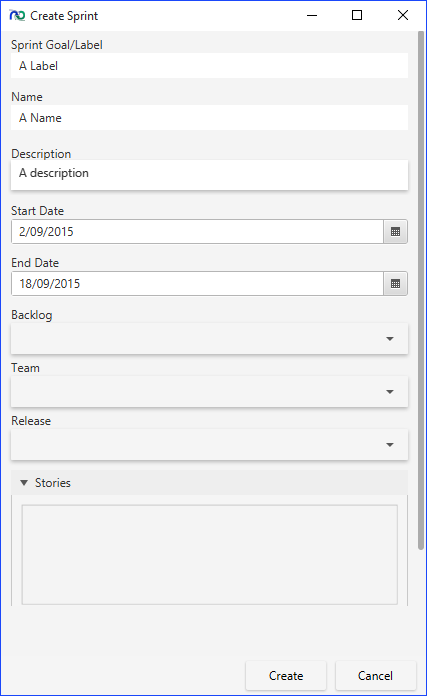
\includegraphics[width=\textwidth]{images/screenshots/sprint1.PNG}
\caption{Creating a Sprint}
\label{fig:new_project}
\end{figure}

You can then add stories to the sprint from the backlog you have assigned it. If you change the backlog you've assigned it too after adding stories it will warn you as it will remove all the stories that you've added to the sprint so far.

Another view that you can access in the sprints editor pane is the all tasks view, this is one of the tabs at the side of the editor. This gives you a view of all the tasks that are in the sprint. These tasks can be filtered by allocated (have people assigned to them) and unallocated (no one is assigned to them). They can also be ordered alphabetically by name, by the story state or their current estimate. Another feature is that you can group them into their corresponding stories.

\begin{figure}[H]
\centering
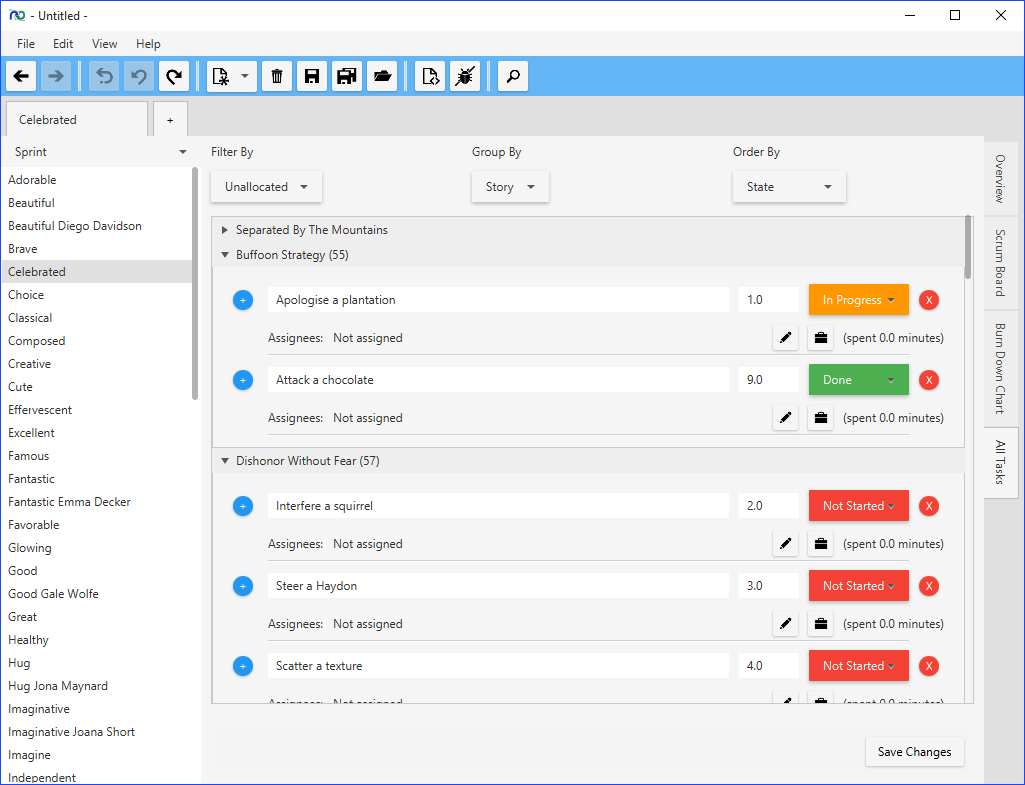
\includegraphics[width=\textwidth]{images/screenshots/sprint2.PNG}
\caption{Viewing all Tasks in a Sprint}
\label{fig:new_project}
\end{figure}